\documentclass{article}
\usepackage[francais]{babel}
\usepackage[utf8]{inputenc} % Required for including letters with accents
\usepackage[T1]{fontenc} % Use 8-bit encoding that has 256 glyphs
\usepackage{pythontex}
\usepackage{amsthm}
\usepackage{amsmath}
\usepackage{amssymb}
\usepackage{mathrsfs}
\usepackage{graphicx}
\usepackage{geometry}
\usepackage{stmaryrd}
\usepackage{tikz}
\usetikzlibrary{patterns}
%\usetikzlibrary{intersections}
\usepackage[cache=false]{minted}
\usepackage{xcolor}

\usepackage{stmaryrd}
%\usepackage{tikz}
%\usetikzlibrary{tikzmark}
\usepackage{empheq}
\usepackage{longtable}
\usepackage{booktabs} 
\usepackage{array}
\usepackage{pstricks}
\usepackage{pst-3dplot}
\usepackage{pst-tree}
\usepackage{pstricks-add}
\usepackage{upgreek}
%\usepackage{epstopdf}
\usepackage{eolgrab}
\usepackage{chngpage}
 \usepackage{calrsfs}
 % Appel du package pythontex 
\usepackage{pythontex}

\usepackage{algorithm2e}
\RestyleAlgo{algoruled}
  \SetKw{KwFrom}{from} 
\newenvironment{algo}{
\begin{algorithm}[H]
\DontPrintSemicolon \SetAlgoVlined}
{\end{algorithm}}



\usetikzlibrary{decorations.pathmorphing}
\def \de {{\rm d}}
\usepackage{color}
\usepackage{xcolor}
\newcommand{\mybox}[1]{\fbox{$\displaystyle#1$}}
\newcommand{\myredbox}[1]{\fcolorbox{red}{white}{$\displaystyle#1$}}
\newcommand{\mydoublebox}[1]{\fbox{\fbox{$\displaystyle#1$}}}
\newcommand{\myreddoublebox}[1]{\fcolorbox{red}{white}{\fcolorbox{red}{white}{$\displaystyle#1$}}}

\usepackage{xcolor}
%\setbeamercolor{background canvas}{bg=lightgray}
\definecolor{LightGray}{gray}{0.9}
\definecolor{monOrange}{rgb}{0.97,0.35,0.04}

 \title{Création de notre première application Vue}
\author{Ibrahim ALAME}
\date{14/02/2023}
\begin{document}
\maketitle

\section{La librairie create-vue}
\subsection{Première utilisation de la librairie {\color{monOrange} create-vue}}
Commencez par créer un dossier à l'emplacement que vous souhaitez. Ouvrez un terminal à l'emplacement du dossier et entrez la commande suivante :
\begin{minted}[
mathescape,
framesep=2mm,
baselinestretch=1.2,
fontsize=\footnotesize,
bgcolor=LightGray,
%linenos
]{bash}
npm init vue@latest
\end{minted}

Cette commande permet d'installer et d'exécuter la dernière version de {\color{monOrange}create-vue} qui permet de lancer la configuration d'une nouvelle application {\color{monOrange} Vue.js}. Lorsque vous entrez la commande pour la première fois vous aurez la demande de confirmation d'installer {\color{monOrange}create-vue }:
\begin{minted}[
mathescape,
framesep=2mm,
baselinestretch=1.2,
fontsize=\footnotesize,
bgcolor=LightGray,
%linenos
]{bash}
Need to install the following packages:
  create-vue@latest
Ok to proceed?
\end{minted}

Vous devrez simplement répondre {\tt y} ou {\tt yes}. Viennent ensuite toutes les questions sur la configuration de l'application. La première est le nom que vous souhaitez donner à votre application :
\begin{minted}[
mathescape,
framesep=2mm,
baselinestretch=1.2,
fontsize=\footnotesize,
bgcolor=LightGray,
%linenos
]{bash}
Project name: › vue-project
\end{minted}

Par défaut, le nom est prérempli avec vue-project mais vous pouvez bien sûr le changer.

La deuxième question est sur l'utilisation de TypeScript :
\begin{minted}[
mathescape,
framesep=2mm,
baselinestretch=1.2,
fontsize=\footnotesize,
bgcolor=LightGray,
%linenos
]{bash}
Add TypeScript? … No / Yes
\end{minted}

Comme nous l'avons vu, choisissez oui.

Ensuite répondez non pour JSX.

Nous n'utiliserons par JSX qui est un langage de template React.

Répondez non pour Vue Router, Pinia, Vitest et Cypress car nous les verrons plus tard dans la formation.

Répondez oui à ESLint, qui permet de contrôler la qualité du code et répondez oui à Prettier pour le formatage du code.

Vous devez en être là :
\begin{center}
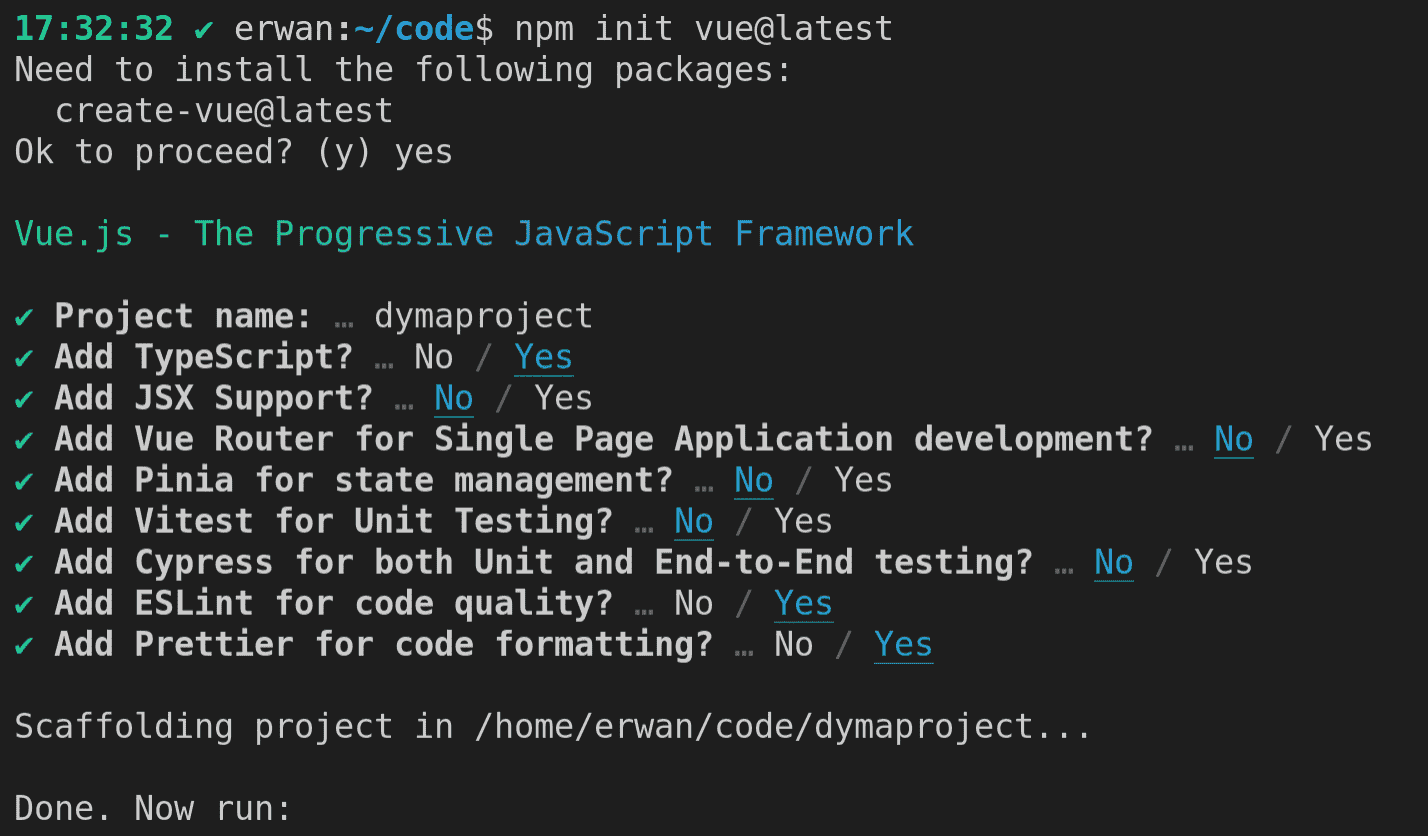
\includegraphics[width=10cm]{images/image04.png}
\end{center}

\subsection{Installation des dépendances}
Pour le moment, create-vue a déclaré toutes les dépendances et les configurations nécessaires en suivant vos options.

Aucune dépendance JavaScript n'a encore été installée par npm.

Pour les installer, il suffit d'ouvrir un terminal et d'aller dans le dossier de votre application, par exemple :
\begin{minted}[
mathescape,
framesep=2mm,
baselinestretch=1.2,
fontsize=\footnotesize,
bgcolor=LightGray,
%linenos
]{bash}
cd dymaproject
\end{minted}

Et ensuite de lancer l'installation des dépendances :
\begin{minted}[
mathescape,
framesep=2mm,
baselinestretch=1.2,
fontsize=\footnotesize,
bgcolor=LightGray,
%linenos
]{bash}
npm install
\end{minted}

\subsection{Utilisation du linter}
Un linter est un outil d'analyse de code qui permet de détecter les erreurs et les problèmes de syntaxe.

La configuration du linter, en l'occurrence ESLint est dans le fichier .eslintrc.cjs :
\begin{minted}[
mathescape,
framesep=2mm,
baselinestretch=1.2,
fontsize=\footnotesize,
bgcolor=LightGray,
%linenos
]{bash}
/* eslint-env node */
require('@rushstack/eslint-patch/modern-module-resolution')

module.exports = {
  root: true,
  'extends': [
    'plugin:vue/vue3-essential',
    'eslint:recommended',
    '@vue/eslint-config-typescript',
    '@vue/eslint-config-prettier/skip-formatting'
  ],
  parserOptions: {
    ecmaVersion: 'latest'
  }
}
\end{minted}

create-vue a donc automatiquement créé la bonne configuration du linter pour une utilisation avec Vue.js.

Pour exécuter le linter avec la configuration faites :

\begin{minted}[
mathescape,
framesep=2mm,
baselinestretch=1.2,
fontsize=\footnotesize,
bgcolor=LightGray,
%linenos
]{bash}
npm run lint
\end{minted}     

Cela exécutera le script lint déclaré dans le fichier package.json.

Pour l'instant il y a bien sûr aucune indication car nous n'avons pas commencé à coder !

Mais exécuter cette commande de temps en temps lors du développement permet d'éviter certaines erreurs et de suivre les recommandations pour les bonnes pratiques en matière de syntaxe (appelées coding style).

\subsection{Lancer le serveur de développement}
Pour lancer le serveur de développement il suffit d'exécuter le script dev :
\begin{minted}[
mathescape,
framesep=2mm,
baselinestretch=1.2,
fontsize=\footnotesize,
bgcolor=LightGray,
%linenos
]{bash}
npm run dev
\end{minted} 

Cela va en fait exécuter vite qui va lancer son serveur de développement.

Vous pourrez ainsi accéder à l'application Vue.js dans votre navigateur à l'adresse http://localhost:3000/.


\end{document}


Le fonctionnement de tous nos cours est similaire. Chaque cours est divisé en chapitres et en leçons.
\subsection{Contenu des leçons}
Chaque leçon comporte une vidéo, un support écrit et un quiz.

La vidéo permet d'avoir une première vue sur l'essentiel de la leçon, et également de voir immédiatement des exemples.

Le cours permet d'approfondir la vidéo et de voir d'autres exemples et ressources pour acquérir une compréhension profonde de la notion.

Le quiz permet de valider la compréhension de la notion. Il n'y a qu'une seule bonne réponse, et vous devez valider le quiz pour passer à la suite. Vous pouvez bien sûr essayer le quiz autant de fois que nécessaire et revoir les parties de cours correspondantes entre temps. En cas d'erreur, des explications vous sont toujours données.

\subsection{Les chats}
Pendant votre formation, vous avez deux moyens de nous joindre à tout moment.

Premièrement, pour les éventuels problèmes avec la plateforme, un paiement ou votre progression que vous rencontreriez, vous pouvez nous contacter sur le chat en bas à droite.

Deuxièmement, pour les questions techniques, vous pouvez les poser à tout moment sur le chat en bas à gauche. La communauté de tous les apprenants, ou nous-mêmes, vous aideront !

\subsection{Prérequis et suite du cours}
Les prérequis de cette formation sont une bonne maîtrise de HTML \& CSS et de JavaScript. Si ce n'est pas le cas, suivez d'abord ces deux formations sur la plateforme.

Une connaissance du langage TypeScript est un plus, même si nous verrons les fondamentaux nécessaires dans la formation. Vous pouvez suivre en parallèle la formation TypeScript pour approfondir.

Nous recommandons également de faire la formation Git, au moins les premiers chapitres si vous ne connaissez pas cet outil.

Après ce cours vous pourriez vouloir devenir développeur Fullstack. Vous pourrez alors suivre par exemple les cours Node.js et MongoDB.

%%%%%%%%%%%%%%%%%%%%%%%%%ù

\section{Introduction à Vue.js}
\subsection{Qu'est ce que Vue.js ?}
Vue.js est un framework permettant de développer des interfaces utilisateur.

Il est développé entièrement en TypeScript depuis sa version 3.

TypeScript est un langage de programmation open source développé par Microsoft. C'est un sur-ensemble syntaxique de JavaScript.

Cela signifie que c'est du JavaScript amélioré, qui permet notamment un typage fort. Il est ensuite transformé en JavaScript. Les navigateurs ne comprennent en effet que les langages HTML, CSS et JavaScript.

Vue.js est fondé sur deux concepts clés : le rendu déclaratif et la réactivité.

Le rendu déclaratif est le fait de décrire le rendu (HTML) en fonction de l'état de l'application (en JavaScript).

La réactivité est le fait que Vue suit les changements d'état dans le code JavaScript et met à jour le DOM de manière optimisée si des changements doivent être faits.

\subsection{Un framework progressif}
L'une des grandes forces de Vue.js est d'être progressif : vous pouvez faire une application très simple sans étape de build juste avec la librairie core, mais vous pouvez aussi faire une application très complexe avec beaucoup d'étapes de build automatisés, une gestion des routes, de l'état de l'application etc.

Nous verrons ainsi notamment les librairies officielles suivantes, qui font partie du framework Vue.js :

Vue Router : permet de gérer la navigation de l'utilisateur dans l'application.

Pinia : permet de gérer l'état de l'application.

Vite : permet de construire l'application (par exemple en transpilant le Sass et CSS ou le TypeScript en JavaScript) et de l'optimiser.

Transpiler signifie convertir dans un autre langage de même niveau (contrairement à la compilation qui transforme du code dans un langage de haut niveau à un langage plus proche du langage machine).

\subsection{Tous les rendus possibles !}
Vue.js permet aujourd'hui de faire des applications de tous les principaux types de rendu :

SPA (Single-Page Application) : le serveur envoie une page HTML avec un lien vers des fichiers JavaScript qui contiennent toute l'application. Le navigateur va charger toute l'application qui va gérer un grand nombre d'opérations comme le routage entre les pages.

SSR (Server Side Rendering) : la page Web est générée par le serveur qui construit le HTML, le CSS et le JavaScript nécessaires en fonction de la requête, pour rendre la page. Pendant ce temps, le navigateur télécharge la SPA qui sera ensuite utilisée. Cela permet aux utilisateurs d'avoir un premier affichage quasi-immédiat sans avoir à attendre le chargement de l'application. Lorsque le SSR est configurée on dit alors que l'application est universelle car elle est rendue à la fois côté serveur et côté client. Nous reviendrons en détail sur ces notions dans la formation.

SSG (Static-Site-Generation / JAMStack ) : toutes les pages sont pré-générées sur le serveur (tout le HTML, le CSS et le JavaScript est générés en amont) et servies au navigateur en fonction des requêtes. C'est utile pour faire de petits sites statiques. Vous pouvez alors utiliser VitePress, la librairie SSG officielle de Vue.

Vous pouvez également faire des applications bureautiques (par exemple avec Electron ou Tauri), des applications mobiles (par exemple avec Ionic ou Quasar) ou encore utiliser WebGL ou développer des applications pour le terminal.

\subsection{Une traction incroyable}
Contrairement à Angular ou React aucun géant du numérique ne se cache derrière Vue.js mais seulement Evan You, et bien sûr de très nombreux contributeurs.

Vue.js a une traction phénoménale ces dernières années : il dépasse les 3 millions de téléchargements par semaine sur npm !

C'est le framework JavaScript qui a le plus d'étoiles sur Github (environ 200 000).

Le framework est aujourd'hui très stable et est utilisé notamment par Laravel (comme framework Javascript par défaut), par GitLab et par PageKit.

En Chine, il s'agit du framework le plus utilisé avec notamment Alibaba, Baidu, Sina Weibo et Xiaomi qui l'utilisent en production.

Nous pouvons donner quelques autres exemples de sites connus faits avec Vue.js : Gitlab, Behance, Upwork, Back Market, Louis Vuitton USA, Ecosia, Google Carreers, plusieurs sites de Microsoft (par exemple Azure for Partners), de très nombreux sites d'Alibaba, Baidu,

\subsection{Vue.js 3}
Vue.js 3 est sorti en septembre 2020 et est devenu la version officielle par défaut en février 2022 (le temps que les autres librairies du framework soient également réécrites).

L'ensemble du framework a été entièrement réécrit en TypeScript et a de bien meilleures performances que la version 2. Il est encore plus léger et optimisé.

Il bénéficie également d'une toute nouvelle API appelée Composition API qui permet de rendre plus facile le développement d'applications complexes.

Vue.js 3 est donc une nouvelle version vraiment différente de la version 2 avec de nombreuses modifications.

Les librairies composants le framework ont également changé : Vite a remplacé Webpack et Pinia a remplacé Vuex par exemple.

\subsection{Avantages}
\subsubsection{Taille}
La librairie Vue.js fait seulement 20kB lorsqu'elle est minimisée et compressée, c'est donc un framework très léger qui se charge instantanément par le client.

\subsubsection{Rapidité}
Les performances de Vue sont excellentes et elles surpassent même celles de React sur le rendu et la mise à jour du DOM.

Vue.js utilise un DOM virtuel pour minimiser le nombre de mutations du DOM nécessaires lors de changements.

Vue.js a des algorithmes de calcul des mutations nécessaires qui s'avèrent plus performants et légers que ceux de React.

\subsubsection{Un framework complet}
Vue comporte tous les éléments pour une application moderne complexe : gestion de la navigation, gestion avancée de l'état, gestion de la construction de l'application de manière optimisée, gestion des rendus (même universel avec le SSR) etc.

Autrement dit, Vue gère tout !

\subsection{Note sur le choix des technologies}
Dans cette formation, nous suivrons l'intégralité des recommandations officielles de Vue.js et / ou d'Evan You pour le choix des technologies.

Pour cette raison, nous utiliserons TypeScript, Vite, le Router Vue, Pinia, Visual Studio Code, Volar, Vue browser devtools, Cypress, Vitest, eslint-plugin-vue et Jest.

Il est possible de ne pas utiliser ces technologies, ou d'en utiliser d'autres mais nous le déconseillons très fortement car ce serait sortir du maintien et de l'évolution souhaitées par les équipes de Vue.js.

%%%%%%%%%%%%%%%%%%%%%%%%%%%%%%%%%%%%%%%%%%%%%%%%%%%%%%%%%

\section{SPA, create-vue et Vite}
\subsection{Les Single Page Applications}
Comme nous l'avons vu précédemment, Vue.js permet de construire des Single Page Applications.

Vous connaissez forcément des SPA : Gmail, Google Analytics, Trello, Dropbox en sont des exemples parmi tant d'autres.

La plupart des frameworks ont adopté cette architecture (Vue, Angular, React, Ember, Meteor etc).

Nous allons maintenant un peu plus détailler les SPA.

Une single page application (SPA) est une application qui fonctionne dans un navigateur sans que l'utilisateur n'ait besoin de recharger la page.

Le principe est de simuler une application hors ligne : pas de rechargement des pages, de la rapidité, pas d'attente supplémentaire dûe au réseau etc.

Les principales caractéristiques de la SPA sont :
\begin{itemize}
\item le rendu est effectué côté client (quand un élément change, la page est modifié grâce aux scripts de l'application chargée côté client).
\item pour fonctionner elle charge en principe une seule fois l'application (HTML, CSS et JavaScript).
\item seules les données sont transmises, si nécessaire, entre le serveur et l'application client (le plus souvent au format JSON).
\item le développement mobile est simplifié car le code backend peut être utilisé que l'application soit Web ou native (iOS, Android).
\item elle est particulièrement adaptée pour stocker les données localement et n'envoyer des requêtes au serveur que lorsque c'est nécessaire.
\end{itemize}

\subsection{La librairie create-vue}
create-vue est la librairie officielle de Vue.js permettant de construire facilement un projet avec Vue.js.

Elle permet de configurer entièrement le framework suivant ses souhaits : utiliser ou non TypeScript, utiliser ou non JSX (le langage de template de Reac), utiliser le Router de Vue, le gestionnaire d'état, la librairie de tests end-to-end etc.

Nous verrons bien sûr à plusieurs reprises comment configurer parfaitement un projet Vue.js en utilisant la librairie.

\subsection{Fonctionnement de Vite}
\begin{center}
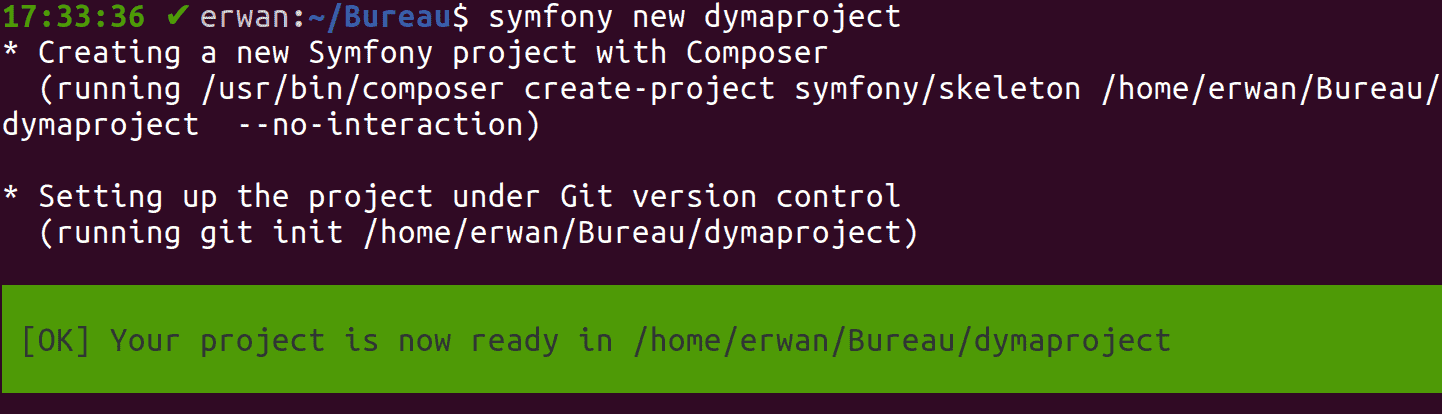
\includegraphics[width=3cm]{images/image1.png}
\end{center}

Vite est un outil de build conçu par le créateur de Vue.js pour remplacer Webpack.

C'est donc tout naturellement que Vue.js recommande aujourd'hui cet outil de build pour réaliser des applications.

Vite vient du français, comme Vue, Evan devant être un amateur de la langue de Molière.

Les deux principales fonctionnalités de Vite sont un serveur de développement et un outil de build pour la mise en production.

Le serveur de développement : permet d'accéder à l'application durant le développement et de recharger ou de réafficher l'application lors de modifications du code de la manière la plus rapide possible.

\subsubsection{La notion de bundler ("empaqueteur")}
\begin{center}
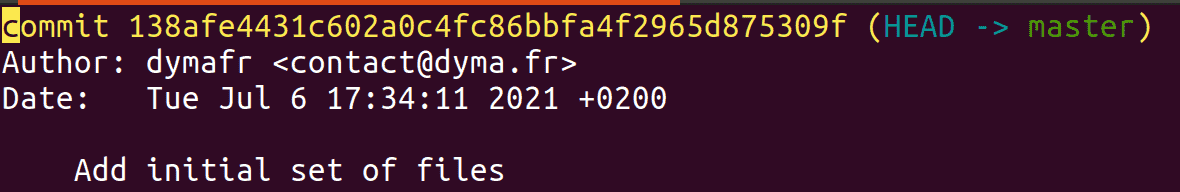
\includegraphics[width=15cm]{images/image2.png}
\end{center}
Un bundle est un regroupement des fichiers JavaScript, HTML et CSS permettant d'accélérer le chargement.

Aujourd'hui, les applications web sont devenues très sophistiquées, c'est pourquoi les frameworks comme Vue.js morcellent le JavaScript, le CSS et le HTML en de nombreux fichiers afin que le code soit maintenable et réutilisable.

Il n'est ainsi pas rare qu'une application complexe dépasse le millier de fichiers.

Les frameworks utilisent des modules JavaScript et gèrent les dépendances de chaque fichier avec import et export. Les fichiers importent les dépendances dont ils ont besoin parmi celles exportées par d'autres fichiers.

Or, les navigateurs Web ont besoin que les fichiers soient organisés d'une certaine manière pour fonctionner. Un bundler permet de les organiser de manière optimisée pour les navigateurs.

Un bundler peut gérer l'arbre de dépendances créés par les imports et exports pour générer des fichiers uniques.

Il réalise également d'autres tâches comme la minification et la compression qui permettent d'obtenir des performances bien supérieures (en rendant le code extrêmement compact et parfois même en le compressant).

\subsubsection{Vite en détail}
Pour le développement, Vite utilise un pré-bundler pour les dépendances. Il permet de bundler les dépendances de 10 à 100 fois plus vite que les outils existants car il est écrit dans un langage plus performant pour ce genre de tâche (Go).

Il utilise également le remplacement à chaud de module (Hot Module Replacement), la mise en cache des dépendances par le navigateur, le rechargement uniquement des modules modifiés et la mise en cache des ressources non modifiées pour accélérer au maximum les rechargements lors des modifications du code en tirant profit des dernières évolutions des navigateurs et du langage JavaScript (principalement les modules EcmaScript, appelés ESM).

Pour la production, Vite va regrouper tous les fichiers JavaScript, HTML et CSS dans un bundle découpé en morceaux (appelés chunks).

La taille des chunks est optimisée pour le chargement par les navigateurs (notamment en tirant profit du nouveau protocole HTTP2) en évitant les allers-retours (requête client / réponse serveur) au maximum.

Les chunks sont également optimisées pour la mise en cache (seules les parties de l'application qui sont modifiées entre deux mises en production auront besoin d'être rechargées par le navigateur).

Elles permettent enfin d'être chargées au bon moment suivant la route pour limiter les chargements inutiles de code côté navigateur (c'est ce qu'on appelle le lazy-loading, nous y reviendrons).

Enfin, Vite permet de tree-shaker l'application : à savoir enlever automatiquement du bundle final, toutes les parties de l'application et les dépendances qui ne sont pas utilisées effectivement par l'application.

Pour le développement et la production, Vite s'assure du pré-traitement (pre-processing) nécessaire pour que l'application puisse être exécutée par les navigateurs.

A titre d'exemple, il va transpiler le TypeScript en JavaScript ou le Sass en CSS.

Vite est donc un outil très puissant qui réalise énormément d'opérations qui sont cachées au développeur pour optimiser la productivité lors de la phase de développement et la performance lors de la production de l'application.

Une fois qu'on a goûté à Vite, il n'est plus possible de s'en passer !

\subsubsection{Qu'est-ce que TypeScript ?}
\begin{center}

\includegraphics[width=3cm]{images/image3.png}
\end{center}

Les projets utilisant JavaScript se sont complexifiés énormément et il est devenu de plus en plus difficile de les maintenir.

Il est compliqué de pouvoir comprendre ce que fait du code JavaScript lorsqu'on arrive sur un projet impliquant de nombreux développeurs.

Il est difficile de savoir ce qu'accepte une fonction et ce qu'elle retourne, et devoir à chaque fois lire les éventuels commentaires pour chaque fonction dans plusieurs fichiers est fastidieux.

De très nombreux langages ou environnement ont tenté d'y remédier, on peut citer notamment : Flow, Dart, Elm, Reason, et Closure.

Mais le seul qui a vraiment conquis l'écosystème et s'est imposé dans une quantité astronomique de projets majeurs est TypeScript.

TypeScript a été créé par Microsoft en 2012, il est depuis le départ un projet open-source.

C'est un langage avec un typage fort et qui transpile en JavaScript.

Transpiler signifie compiler vers un langage de même niveau.

Il est conçu comme une addition pour faire de JavaScript un langage qui scale en ajoutant des types.

Ses avantages immédiats sont :
\begin{enumerate}
\item  Du code beaucoup plus lisible.
\item  Du code beaucoup plus maintenable.
\item  Beaucoup de bugs en moins grâce au compilateur.
\end{enumerate}


Depuis la version 3 de Vue.js, le framework entier est codé en TypeScript et l'équipe recommande fortement l'utilisation de TypeScript.

Si l'utilisation de TypeScript peut paraître fastidieuse au départ c'est un investissement extrêmement lucratif ! Les gains de productivité sont énormes.

Dans la formation nous utiliserons donc TypeScript en vous présentant toutes les bases du langage nécessaires. Si vous voulez ensuite aller plus loin, vous pourrez simplement suivre la formation TypeScript sur la plateforme.

%%%%%%%%%%%%%%%%%%%%%%%%%%%%%%%%%%%%%%%%%%%%%%%%%%%%%%%%%%%%%%%

\section{Environnement GNU/Linux}
\subsection{Installation de Node.js avec node version manager :}
nvm permet d'installer et d'utiliser plusieurs versions de Node.js localement. C'est intéressant si vous avez plusieurs projets à des versions différentes.

Installez nvm :

\begin{minted}[
mathescape,
framesep=2mm,
baselinestretch=1.2,
fontsize=\footnotesize,
bgcolor=LightGray,
%linenos
]{bash}
wget -qO- https://raw.githubusercontent.com/nvm-sh/nvm/v0.39.1/install.sh | bash
\end{minted}

Collez les commandes suivantes :

\begin{minted}[
mathescape,
framesep=2mm,
baselinestretch=1.2,
fontsize=\footnotesize,
bgcolor=LightGray,
%linenos
]{bash}
export NVM_DIR="$([ -z "${XDG_CONFIG_HOME-}" ] && printf %s "${HOME}/.nvm" || printf %s "${XDG_CONFIG_HOME}/nvm")"
[ -s "$NVM_DIR/nvm.sh" ] && . "$NVM_DIR/nvm.sh" # This loads nvm
\end{minted}

Installez Node.js LTS :

\begin{minted}[
mathescape,
framesep=2mm,
baselinestretch=1.2,
fontsize=\footnotesize,
bgcolor=LightGray,
%linenos
]{bash}
nvm install --lts
\end{minted}

\subsection{Installation de Node sans nvm}
Ouvrez un terminal et entrez la commande suivante qui va installer la version LTS de Node.js :
\begin{minted}[
mathescape,
framesep=2mm,
baselinestretch=1.2,
fontsize=\footnotesize,
bgcolor=LightGray,
%linenos
]{bash}
curl -fsSL https://deb.nodesource.com/setup_lts.x | sudo -E bash -
sudo apt-get install -y nodejs
\end{minted}

Vérifiez l'installation :
\begin{minted}[
mathescape,
framesep=2mm,
baselinestretch=1.2,
fontsize=\footnotesize,
bgcolor=LightGray,
%linenos
]{bash}
node -v
\end{minted}

\subsection{Installation de VS Code avec snap sur Ubuntu}
Pour installer l'éditeur VS Code sur Ubuntu, nous vous recommandons d'utiliser snap.

Ouvrez un terminal et faites simplement :
\begin{minted}[
mathescape,
framesep=2mm,
baselinestretch=1.2,
fontsize=\footnotesize,
bgcolor=LightGray,
%linenos
]{bash}
snap install code
\end{minted}

\subsection{Installation de VS Code avec l'installeur}
Si vous êtes sur une autre distribution ou que vous ne souhaitez pas utiliser snap, vous pouvez également utiliser l'installeur.

Il vous suffit de le télécharger ici.

\subsection{Ouvrir un terminal dans VS Code}
Pour ouvrir la vue "Terminal" sur VS Code vous pouvez au choix :

Utiliser Ctrl+`. Si le raccourci ne fonctionne pas. Allez dans le menu File > Preferences > Keymaps. Ensuite recherchez view toggle terminal. Et choisissez un raccourci puis faites Entrée. Nous recommandons Ctrl et la touche la plus à gauche juste sous la touche d'échappement.

Aller dans le menu View > Terminal.

Aller dans le menu Terminal > new terminal.

Tapez Ctrl+Shift+P puis tapez Toggle terminal puis entrée.

Installation d'extensions VS Code
Allez dans l'onglet extension sur VS Code.

Recherchez et installez Volar, TypeScript Vue Plugin (Volar) et Material Icon Theme.
%%%%%%%%%%%%%%%%%%%%%%%%%%%%%%%%%%%%%%%%%%%%%%

\section{Environnement macOS}
\subsection{Installation de Node.js}
Dans le cours vous aurez besoin d'installer des dépendances JavaScript, appelées packages, nous vous conseillons donc d'installer npm qui est le gestionnaire de dépendances de Node.js.

Si vous n'avez pas npm, installez Node.js (qui comprend npm) : ici en sélectionnant l'installeur MacOS.

Si vous préférez utiliser homebrew, ouvrez un terminal et faitres :

\begin{minted}[
mathescape,
framesep=2mm,
baselinestretch=1.2,
fontsize=\footnotesize,
bgcolor=LightGray,
%linenos
]{bash}
brew install node
\end{minted}

\subsection{Installation de VS Code}
Pour installer l'éditeur VS Code, avec l'installeur télécharger le ici.

\subsection{Ouvrir un terminal dans VS Code}
Pour ouvrir la vue "Terminal" sur VS Code vous pouvez au choix :

Utiliser Ctrl+`. Si le raccourci ne fonctionne pas. Allez dans le menu File > Preferences > Keymaps. Ensuite recherchez view toggle terminal. Et choisissez un raccourci puis faites Entrée. Nous recommandons Ctrl et la touche la plus à gauche juste sous la touche d'échappement.

Aller dans le menu View > Terminal.

Aller dans le menu Terminal > new terminal.

Tapez Ctrl+Shift+P puis tapez Toggle terminal puis entrée.

\subsection{Installation d'extensions VS Code}
Allez dans l'onglet extension sur VS Code.

Recherchez et installez Volar, TypeScript Vue Plugin (Volar) et Material Icon Theme.

\end{document}





